\section{Background}
The target audiences of the proposed tool is domain experts who develop learning model for natural language processing tasks. Therefore, certain domain specific background knowledge is required to fully understand and appreciate the technique discussed in this paper. In this section, we first explain the natural language inference (NLI) task and how it fit into the grand challenges in NLP. Then, we examine the common architecture characteristics shared by many state-of-the-art neural network models. Finally, we discuss the role the attention plays in the model and why attention is closely tided to model interpretability.

\subsection{Natural Language Inference}
\label{sec:languageInference}
Natural Language Inference~\cite{DaganRothSammons2013} is an important machine understanding task in NLP.
The problem definition is to classify the relationship between a premise (\textbf{P}) sentence and a hypothesis (\textbf{H}) sentence. 
The prediction must fall in one of three categories: $\{Entailment, Contradiction, Neutral\}$.
$Entailment$ refers to that the textual information of hypothesis is embedded in premise;
$Contradiction$ means the textual of hypothesis opposes that of premise;
and $Neutral$ implies no conclusion can be made on either $Entailment$ or $Contradiction$.
A simple example is illustrated in Table.~\ref{table:NLI}.

\begin{table}[htbp]
\label{table:NLI}
\centering
\caption{An illustration of natural language inference.}
 \begin{tabular}{c | c c c c} 
 \hline
  P / H & sentences & entail & contradict  & neutral \\ [0.5ex] 
 \hline
 premise & Jim ate an apple. &  -  &  -  & - \\ 
 hypothesis & Jim ate a Fuji apple. &   &  & \checkmark \\
 hypothesis & Jim ate fruits. & \checkmark &   &  \\
 hypothesis & Jim ate an banana. &  & \checkmark & \\
 hypothesis & Tom ate an apple &  &  & \checkmark \\
 %\hline
 %premise & Facebook's IPO electrified the general public. &  -  &  -  & - \\ 
 %hypothesis & Facebook went public. & \checkmark   &  &  \\
 %hypothesis & General Electric went public. &  &   & \checkmark \\
 %hypothesis & People ignored Facebook's IPO. &  & \checkmark & \\
 
 \hline
\end{tabular}
\end{table}

However, in real word, the task can be quite challenging, especially for learning algorithms. Take the following sentences as an example (here \textbf{P} refer to premise, \textbf{H} refer to hypothesis):  (\textbf{P}) Facebook's IPO electrified the general public. (\textbf{H1}) Facebook went public. (\textbf{H2}) General Electric went public. (\textbf{H3}) People ignored Facebook's IPO. The literal semantic similarity between ``Electric'' and ``electrified'' will like trick the model to predict \textbf{H2} as \emph{entailment}. The model likely will also not be able to understand the link between ``went public'' and ``IPO'', therefore, mistake \textbf{H1} as \emph{neutral}.

\shusen{How does the NLI related to the other challenges in NLP}
The grand challenge in Natural Language Processing (NLP) is to have machine to acquire
deep comprehension of textual information. Major tasks include Natural Language Inference,
Machine Translation, Questions Answering, Summarization, and etc.
Recently, neural networks models have performed strongly on these tasks.
%
Therefore, making sense and explaining predictions made by deep neural networks is not only
essential for validating and improving the model, but also becoming a necessity with
increasing demands for model accountability (e.g., what is the evidence for making the decision)
and model fairness (e.g., is the prediction affected by the bias in the training data).
%
Recently ~\cite{BowmanAngeliPotts2015} proposed a large dataset for this task. We will examine
the decomposable attention model~\cite{parikh2016emnlp} on this dataset with perturbation.

% Recently, with the wide adoption of long-short term memory
% (LSTM) network and the introduction of attention mechanism,
% neural network based model have dominated nearly all linguistic tasks
% and thoroughtly refreshed many baseline performances.
% %
% However, the disruptive advance also brings enormous challenges.
% Netural network work based on has long been critizied for their opaque nature,
% and often been regarded as back box approach.
% Due to the opaque nature of the neural network model, interpret and making sense
% of many internal model mechanisms can be extremely challenging.

% \subsection{Neural Network Primer}

\begin{figure}[htbp]
\centering
\vspace{-2mm}
 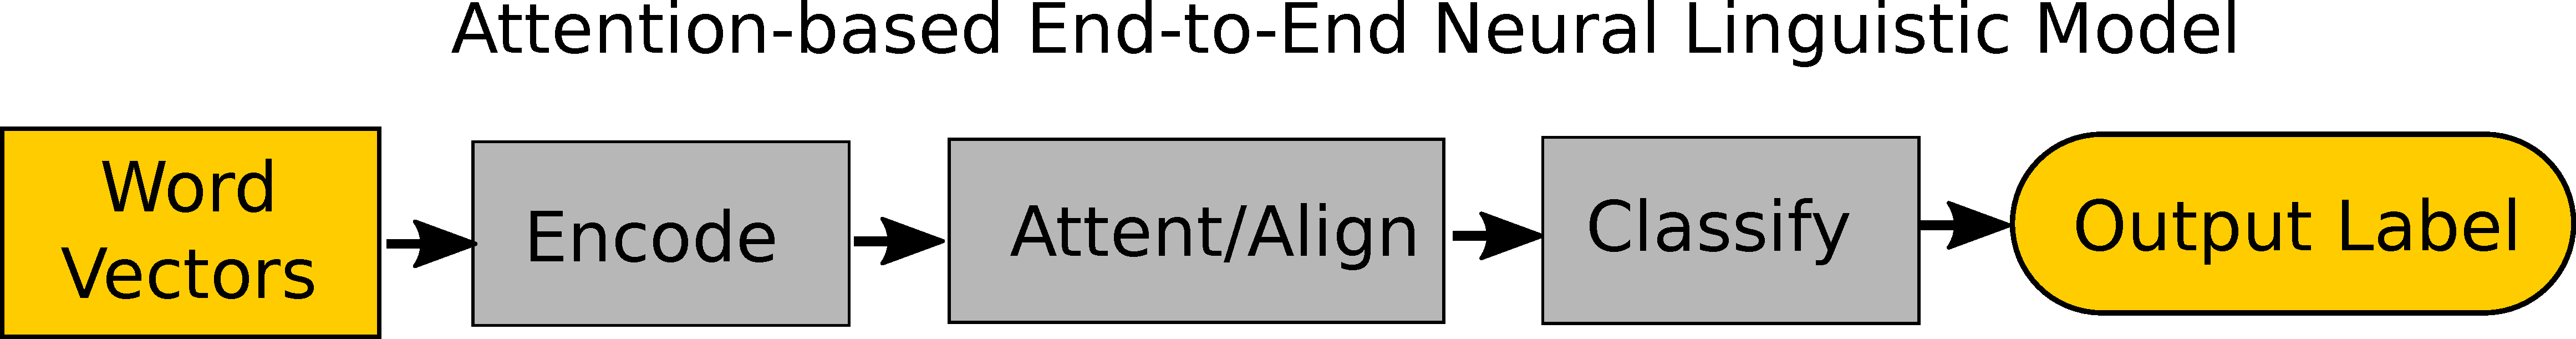
\includegraphics[width=1.0\linewidth]{end2end}
 \caption{End-to-end attention based model.}
\label{fig:modelPipeline}
\end{figure}

\subsection{Neural Network Model in NLP}
\shusen{neural linguistic models?}

\shusen{What is the basic understanding of neural network What is the end-to-end}

% \subsection{Interprebilty Challenges}
Compared with Conputer Vision, the discrete nature of words and sentences
presents additional challenge for
interpreting the model, since many visualization technique often employed
for images rely on continuous nature of the input space (e.g., one can interpolate
real values much easier than interplolate between words/sentences).
%
On the other hand, a majority of recent NLP neural networks share the nature of
end-to-end model, where the entire model operates as a black-box that takes
vectorized input and yields final prediction for a specific task.
Therefore, to study the inside of end-to-end neural models, it is important to
explore the interaction between intermediate representations and predictions.

\subsection{Attention Mechansim}
\label{sec:attention}
The introduction of attention mechanism~\cite{bahdanau2014neural} allows
pairwise interaction between hidden states. This interaction can be naturally explained
as a form of alignment which exposes an interpretable layer in end-to-end neural networks.
Recently attention has contributed to many strongly-performed NLP models
~\cite{parikh2016emnlp},~\cite{rush2015neural},~\cite{yang2016hierarchical},
~\cite{seo2016bidirectional},~\cite{schwartz2017high}.
We will focus on its application in Natural Language Inference task as proposed in~\cite{parikh2016emnlp}.
However notice that our visualization can be generalized to other attention models as well.

\begin{figure}[htbp]
\centering
\vspace{-2mm}
 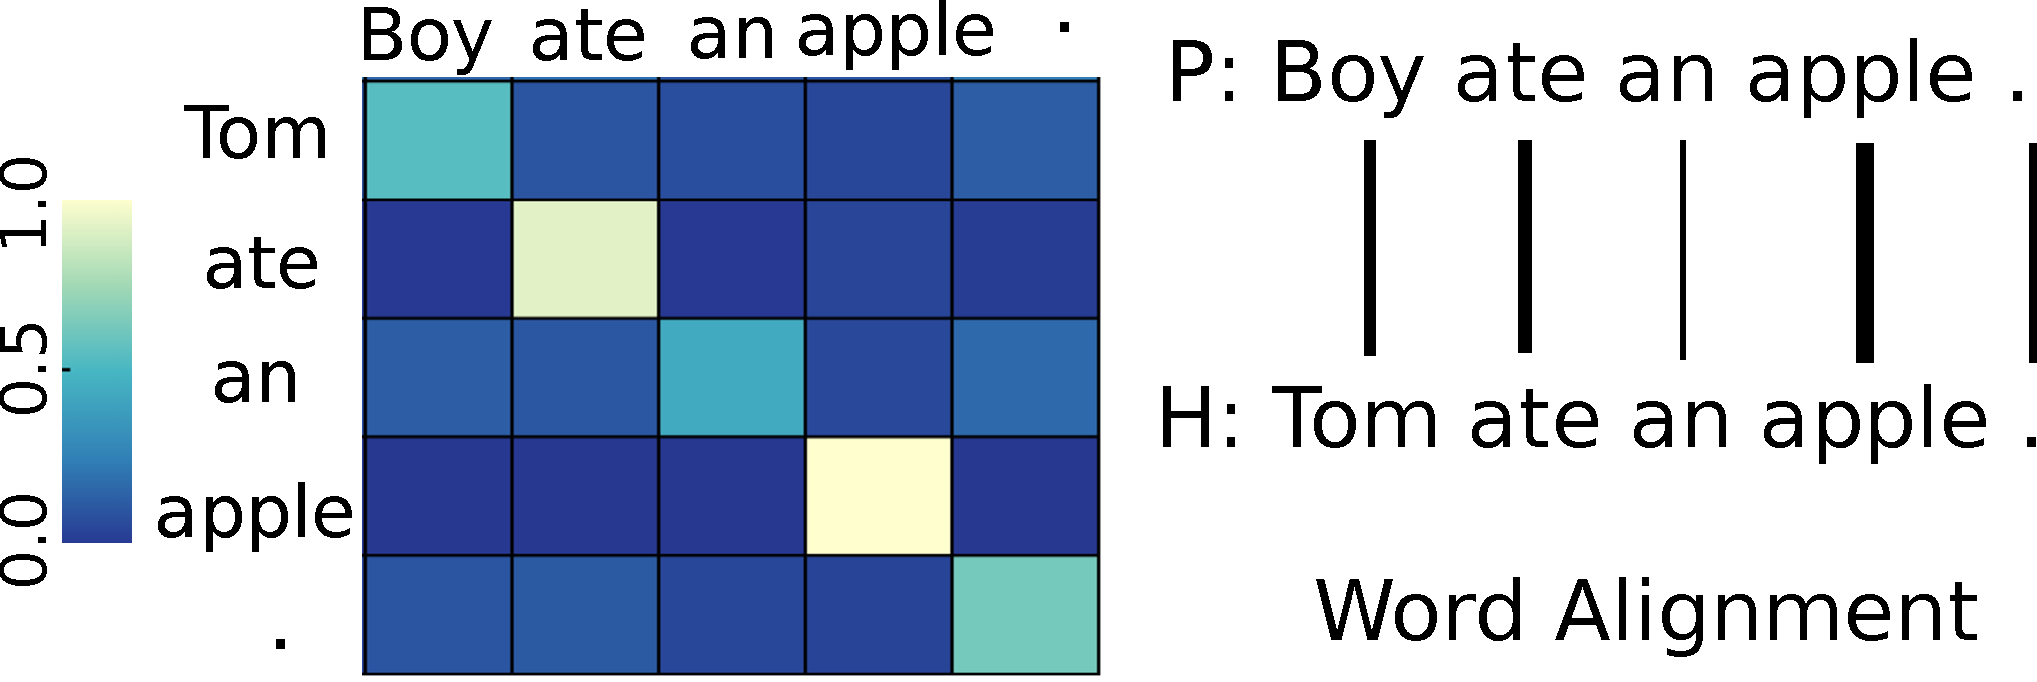
\includegraphics[width=0.9\linewidth]{attentionIllustration}
 \caption{Attention illustrate. The soft alignment between two sentences.}
\label{fig:attention}
\end{figure}

% \begin{itemize}
%     \item what is the textaul entailment problem
%     \item the importance of textual entailment problem
%     \item how easily can the visualization method extends other NLP problem
% \end{itemize}
